\documentclass[UTF8, 11pt, a4paper]{article}
\usepackage[cm]{sfmath}
\usepackage{tabularx}
\def\arraystretch{1.3}
\usepackage[a4paper, top=3.18cm,bottom=3.81cm,left=2.54cm,right=2.54cm]{geometry}
\usepackage{indentfirst}
\setlength{\parskip}{6pt}
\XeTeXlinebreaklocale "zh"
\usepackage{graphicx}
\usepackage[normalem]{ulem}

\usepackage{fontspec}
\setmainfont{思源黑体}
\SetSymbolFont{largesymbols}{normal}{OMX}{iwona}{m}{n}
\setmonofont{Source Code Pro}

\begin{document}
\section*{箱子 / Hako}

\subsection*{描述}
Nuko 在草坪上捡到了一个箱子,想必是某只猫掉下的。

这个箱子里装满了一种水果。Nuko 当然知道它是什么啦!%
不过 Mafu 并不知道,于是又跑来找你帮(ma)忙(fan)了……

\subsection*{输出 \makebox[0.5em]{} \small{hako.out}}
你需要尽可能准确地猜出这种水果名字在正确语言里的正确拼法。%
这种水果的名字包含五个字母,\uwave{每个字母都在 A--N 范围内}。

这是一道(伪)提交答案题。%
程序不必读入任何数据,直接向输出文件中写入即可。

\begin{itemize}
    \item 第 1 行:五个字母(大小写均可),表示你的一次猜测。
\end{itemize}

\subsection*{反馈 \makebox[0.5em]{} \small{hako.feedback}}
对于每次猜测,测评系统会给出一定反馈以帮助你进行下一次猜测。
\begin{itemize}
    \item 如果格式不正确,将给出提示;
    \item 如果格式正确,将给出下列信息:
    \begin{itemize}
        \item 五个位置中有多少个位置上的字母和答案中相同;
        \item 除去正确的位置上的字母,在本次猜测中还有多少个%
            \uwave{不同的}字母在答案中出现过。
    \end{itemize}
\end{itemize}

\subsection*{样例}
\begin{table}[h]\centering
\begin{tabularx}{0.8 \textwidth}{|X|X|}
\hline
\texttt{\textbf{hako.out}} & \texttt{\textbf{hako.feedback}} \\ \hline
{\ttfamily
FACED
} & {\ttfamily
$X$ positions fully matched;\newline
extra $Y$ distinct letters present in your guess.
}
\\ \hline
\end{tabularx}\end{table}

\subsection*{评分}
本题满分为 10 分,提交限制次数为 30 次。

每次格式正确的提交的得分,等于正确位置个数的 2 倍。%
最终本题的得分是所有提交中得分的最大值。

\subsection*{限制}
\begin{itemize}
\item 时间:1.0 秒
\item 内存:32 MiB
\end{itemize}

\begin{figure}[h]\centering
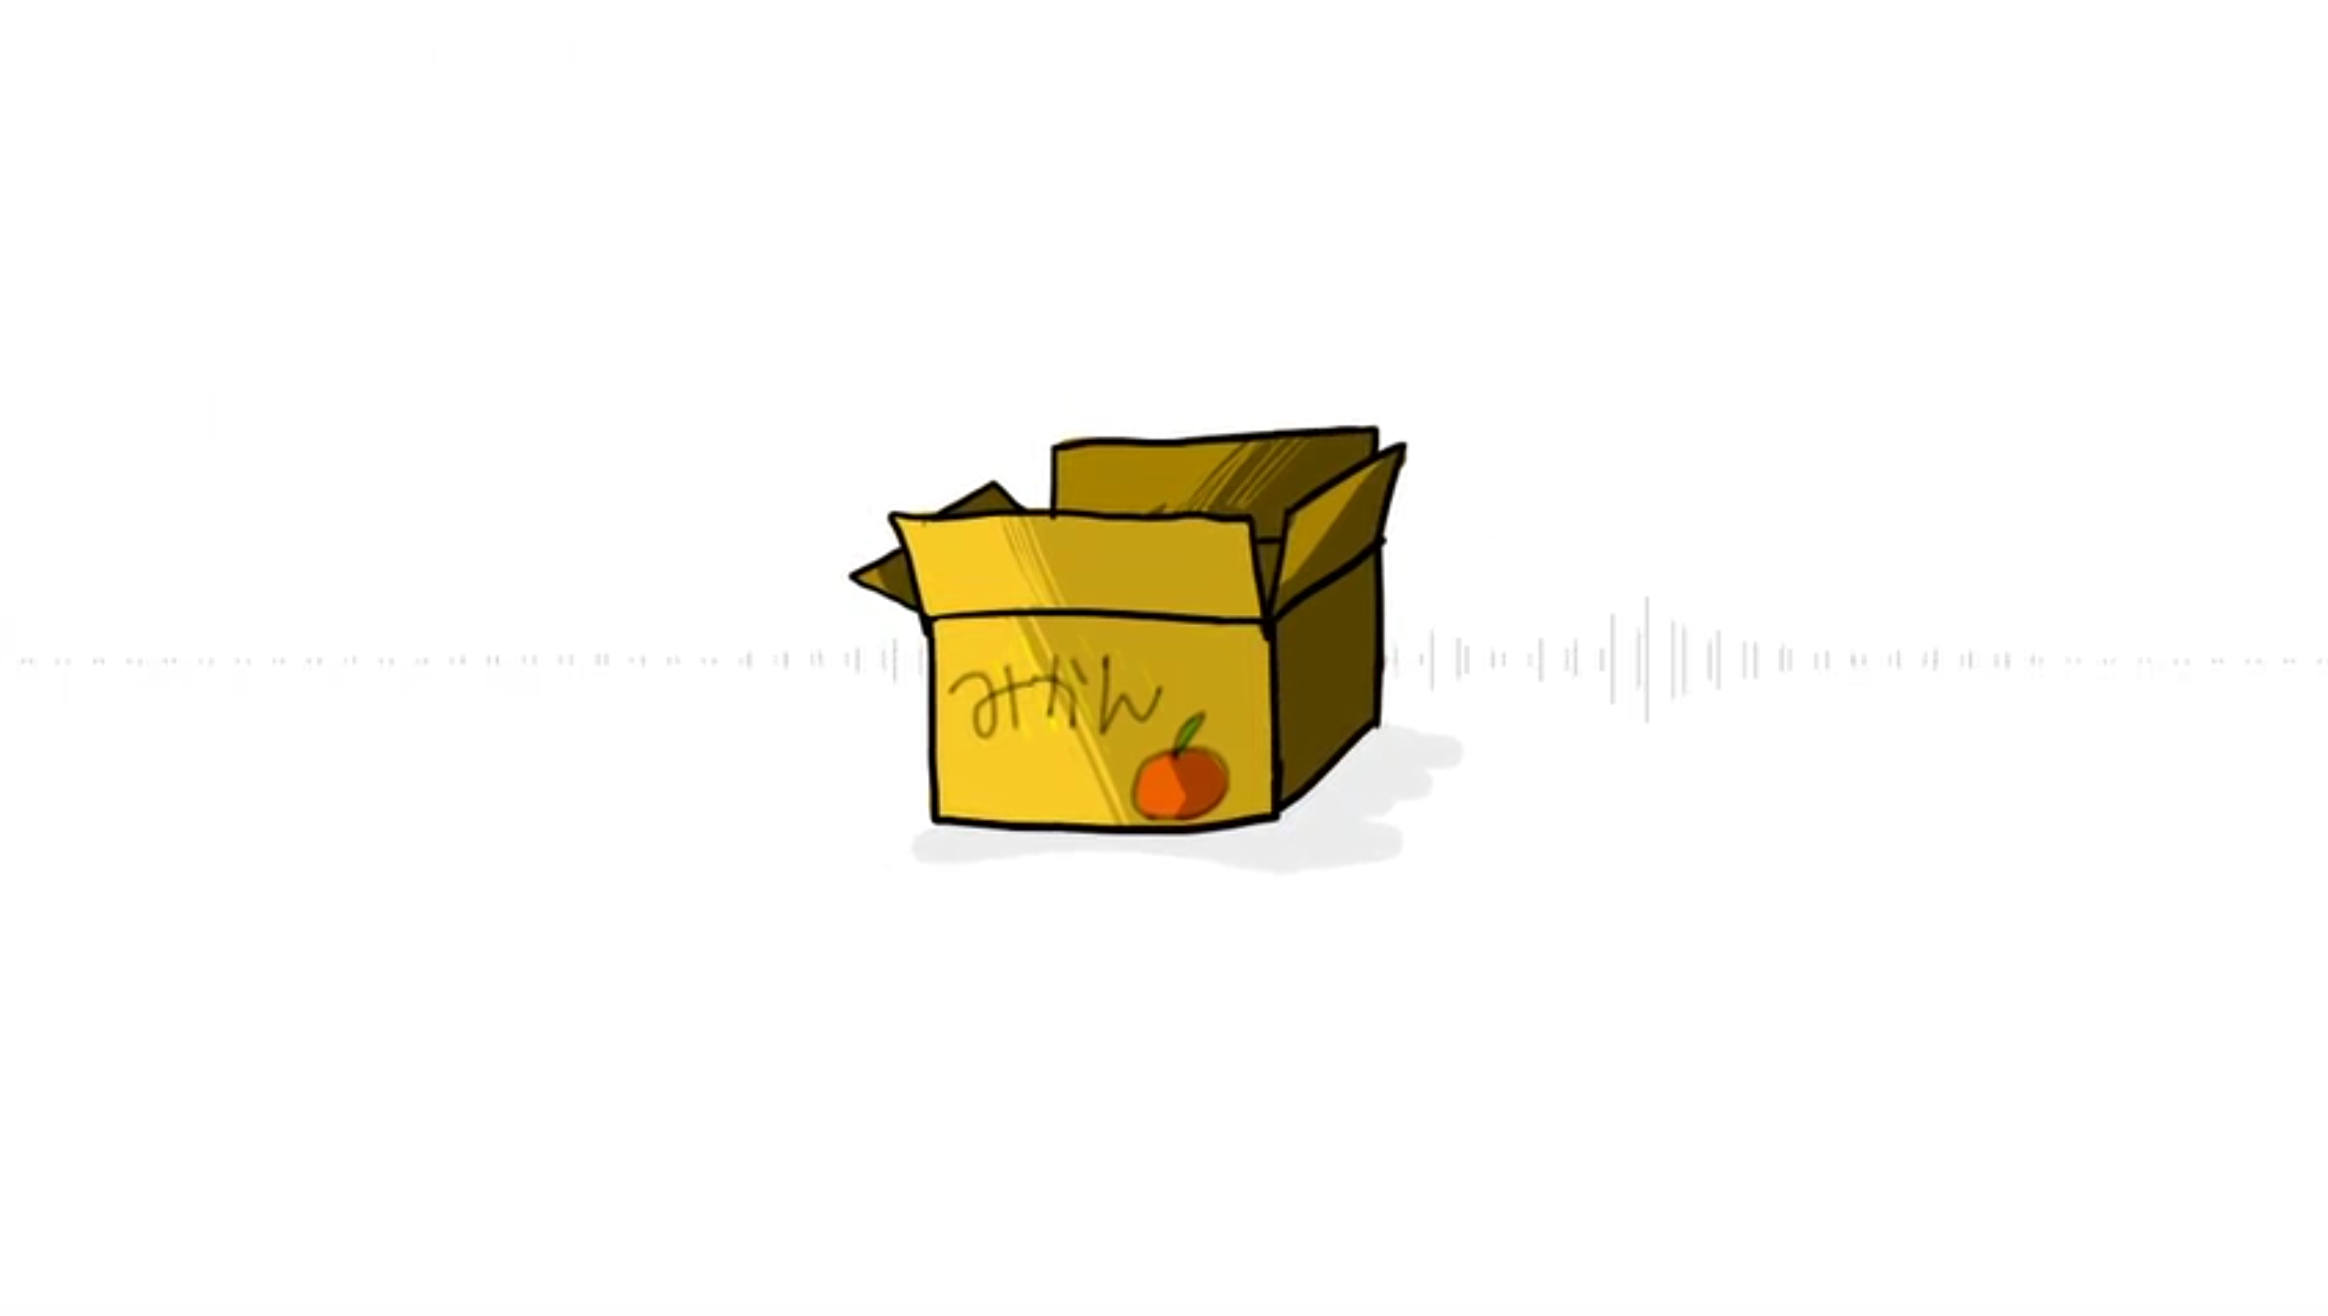
\includegraphics[width=0.6 \textwidth]{hako.png}
\end{figure}

\end{document}

